\documentclass{ximera}
\graphicspath{     %% setup a global graphics path
{./}               %% look in the same-level directory
{./pictures/}      %% look in graphics
{../pictures/}     %% look up one directory, then in graphics
%{../../pictures/} %% look up two directories, then in graphics
}

\author{Zack Reed}
%borrowed from Ana Davis
\title{Decompositions and Orthonormal Bases}
\begin{document}
\begin{abstract}


\end{abstract}
\maketitle

\subsection*{Matrix Multiplication and Projection}

So far, we've had one main way of understanding matrix-vector multiplication:

\begin{enumerate}
   \item Linear Transformation: A matrix $A$ transforms a vector $\vec{v}$ by the product $A\vec{v}$. If $\vec{a}_i$ are the columns of $A$ and $v_i$ are the coordinates of $\vec{v}$, then the the transformed vector $A\vec{v}$ is the linear combination of the columns of $A$ with the coordinates of $\vec{v}$. That is, 
   
   $$A\vec{v}=v_1\vec{a}_1+v_2\vec{a}_2+\ldots+v_n\vec{a}_n.$$
\end{enumerate}

and three main ways of understanding matrix-matrix multiplication:

\begin{enumerate}
   \item Linear Transformation: An $m\times n$ matrix $A$ represents a linear transformation from $\RR^n$ to $\RR^m$, and an $n\times k$ matrix $B$ represents a linear transformation from $\RR^k$ to $\RR^n$. The matrix product $A*B$ is an $m\times k$ matrix that represents a linear transformation from $\RR^k$ to $\RR^m$.
   \item Column-wise matrix-vector multiplication: If $A$ is an $m\times n$ matrix and $B$ is an $n\times k$ matrix with columns $\vec{b}_i$, then the matrix product $A*B$ is an $m\times k$ matrix whose columns are the matrix-vector products $A\vec{b}_i$. That is:
   
   $$A*B=\left[A\vec{b}_1, A\vec{b}_2, \ldots, A\vec{b}_n\right].$$
   \item Entry-wise multiplication: Let $A$ be an $m\times n$ matrix and $B$ be an $n\times k$ matrix. The product $A*B$ is an $m\times k$ matrix whose entries are given by
 
   $$(AB)_{ij}=\sum_{k=1}^n A_{ik}B_{kj}.$$
\end{enumerate}

Now, we gain a new understanding of both, related to the dot product. First we will look more closely at the entry-wise matrix multiplication formula in the light of linear combinations and the dot product, and then we will extend this to the column-wise matrix-vector multiplication of matrices.

First, le'ts take a look at the entry-wise definition. The key formula is that the $i,j$ entry of the matrix is given by 

$$(AB)_{ij}=\sum_{k=1}^n A_{ik}B_{kj}.$$

The key thing to note is that the term $A_{ik}$ comes from the $i$th row, $k$th column of $A$, and that $B_{kj}$ comes from the $k$th row, $j$th column of $B$. Let's play this out on the dot product $\vec{u}\cdot\vec{v}$.

\begin{example}
   If $\vec{u}=\begin{bmatrix}
      u_1\\u_2\\\vdots\\u_n
   \end{bmatrix}$ and $\vec{v}=\begin{bmatrix}
      v_1\\v_2\\\vdots\\v_n
   \end{bmatrix}$ are two vectors, then the dot product $\vec{u}\cdot\vec{v}$ is the matrix multiplication

   $$\vec{u}\cdot\vec{v}=\left[u_1 u_2 \ldots u_n\right]\begin{bmatrix}
      v_1 \\ v_2 \\ \vdots \\ v_n
   \end{bmatrix}=\sum_{k=1}^nu_kv_k.$$


\end{example}

Since in the dot product $\vec{u}$ is a $1\times n$ matrix and $\vec{v}$ is a $n\times 1$ matrix, the dot product is the same as the calculation of the $i,j$ term in the product $(AB)_{ij}$!

So, one way of viewing matrix multiplication is that every entry of the product $(AB)_{ij}$ is the dot product of the $i$th row of $A$ with the $j$th column of $B$. This is a better explanation of the matrix multiplication entry-wise formula.

Now, this also gives us a quicker way to do the dot products of many vectors at once!

\subsection*{Orthogonal Projection From Matrix Multiplication}

Suppose you have $m$ $n$-dimensional vectors $\lbrace \vec{u}_1, \vec{u}_2, \ldots, \vec{u}_m\rbrace$ making column-wise the matrix $M$, and $k$ $n$-dimensional vectors $\lbrace \vec{v}_1, \vec{v}_2, \ldots, \vec{v}_k\rbrace$ making the matrix $N$. 

Either the products $M^T*N$ or $N^T*M$ will give you the $k\times n$ (or $n\times k$) dot products of each vector in $M$ with each vector in $N$.

Let's try it out!

\begin{example}

   The matrix $M=\begin{bmatrix}
         .714 & -.698 &.059\\-.645&-.688&-.332\\.273&.199&-.941
      \end{bmatrix}$ has columns $\vec{m}_1$, $\vec{m}_2$ and $\vec{m}_3$ from the orthonormal basis for $\RR^3$ constructed in the previous section. 

   Let's take the dot product of these three vectors with a random vector in $\RR^3$, say, $\vec{v}=\begin{bmatrix}
      1, 2, 3
   \end{bmatrix}$. 

   To do this, we take $M^T\vec{v}$ so that the resulting $3\times 1$ vector gives the three dot products of the columns of $M$ with $\vec{v}$.

   \begin{verbatim}
   M=[.714 -.698 .059;
   -.645 -.688 -.332;
   .273 .199 -.941]
   v=[1;2;3]
   M_dot_vs=M'*v
   \end{verbatim}
   
   This gives

   $$M^T\vec{v}=\begin{bmatrix}
      \answer[tolerance=.01]{.24}\\\answer[tolerance=.01]{-1.28}\\\answer[tolerance=.01]{-3.4280}
   \end{bmatrix}.$$

   This means that $\vec{m}_1\cdot \answer[tolerance=.01]{.24}$, $\vec{m}_2\cdot\answer[tolerance=.01]{-1.28}$, and $\vec{m}_3\cdot\vec{v}=\answer[tolerance=.01]{-3.4280}$.

   Suppose we wanted to find the dot product of two vectors $\vec{u}=\begin{bmatrix}
   3\\-1\\2
   \end{bmatrix}$ and $\vec{w}=\begin{bmatrix}
      -2\\3\\3
   \end{bmatrix}$, we could form a matrix $N=\begin{bmatrix}3&-2\\-1&3\\2&3
   \end{bmatrix}$ and similarly calculate the dot products of these two vectors with each basis vector in $M$. 

   This yeilds the dot products

   $$M^T*N=\begin{bmatrix}
      \answer[tolerance=.01]{3.33}&\answer[tolerance=.01]{-2.54}\\\answer[tolerance=.01]{-1.01}&\answer[tolerance=.01]{-.07}\\
      \answer[tolerance=.01]{-1.37}&\answer[tolerance=.01]{-3.94}
   \end{bmatrix},$$

   Which gives us the dot products $\vec{m}_3\cdot w=\answer[tolerance=.01]{-3.94}$, $\vec{m}_2\cdot v=\answer[tolerance=.01]{-1.01}$ and $\vec{m}_1\cdot w=\answer[tolerance=.01]{-2.54}$.

\end{example}

As it turns out, dot products with orthonormal bases are particularly special, further extending the utility of having orthonormal bases.

We began with the motivation of orthogonally decomposing vectors $\vec{v}$ into parallel and perpendicular vectors $\vec{v}_\parallel$ and $\vec{v}_\perp$ such that $\vec{v}=\vec{v}_\parallel+\vec{v}_\perp$, where $\vec{v}_\parallel$ is in the direction of the unit vector $\vec{u}$ and $\vec{v}_\perp$ is orthogonal to $\vec{u}$, as in the following diagram:

\begin{center}
   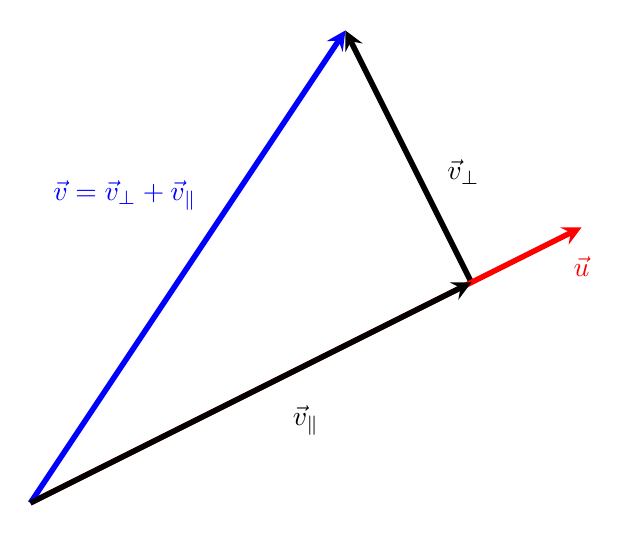
\begin{tikzpicture}
    \draw[line width=2pt,black,-stealth](3.6, 0.8)--(2,4);
    \node[black] at (3.5, 2.2)   (a) {$\vec{v}_{\perp}$};
   \node[black] at (1.5, -0.95)   (b) {$\vec{v}_{\parallel}$};
    \node[red] at (5, 1)   (c) {$\vec{u}$};
    \node[blue] at (-0.8, 1.9)   (d) {$\vec{v}=\vec{v}_{\perp}+\vec{v}_{\parallel}$};
    \draw[line width=2pt,red,-stealth]  (-2,-2)--(5, 1.5);
     %\draw [line width=1pt, red, stealth]  (-3,-2.5)--(5, 1.5);
  \draw[line width=2pt,blue,-stealth](-2, -2)--(2,4);
  \draw[line width=2pt,black,-stealth](-2, -2)--(3.6, 0.8);
  \end{tikzpicture}
   
  \end{center}

What has been thus far left unsaid, was that if $\vec{u}_\perp$ is the unit vector perpendicular to $\vec{u}$, then $\vec{u}_\perp$ and $\vec{u}$ form an orthonormal basis for $\RR^2$.

Moreover, if we do the same orthogonal decomposition of $\vec{v}$, but for $\vec{u}_\perp$ instead of for $\vec{u}$, and then put both diagrams together, we would get the following diagram:

\begin{center}
   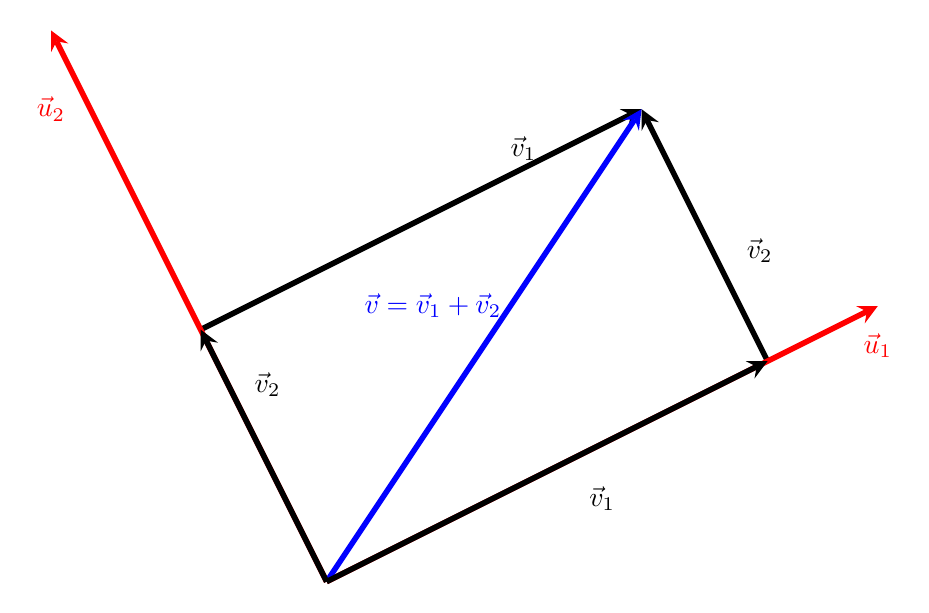
\begin{tikzpicture}
    \draw[line width=2pt,black,-stealth](3.6, 0.8)--(2,4);
    \draw[line width=2pt,black,-stealth](-3.6, 1.2)--(2,4);
    \node[black] at (3.5, 2.2)   (a) {$\vec{v}_2$};
    \node[black] at (-2.75, .5)   (a) {$\vec{v}_2$};
   \node[black] at (1.5, -0.95)   (b) {$\vec{v}_1$};
   \node[black] at (.5, 3.5)   (b) {$\vec{v}_1$};
    \node[red] at (5, 1)   (c) {$\vec{u}_1$};
    \node[red] at (-5.5,4) (d) {$\vec{u}_2$};
    \node[blue] at (-.65, 1.5)   (d) {$\vec{v}=\vec{v}_1+\vec{v}_2$};
    \draw[line width=2pt,red,-stealth]  (-2,-2)--(5, 1.5);
    \draw[line width=2pt,red,-stealth]  (-2,-2)--(-5.5, 5);
     %\draw [line width=1pt, red, stealth]  (-3,-2.5)--(5, 1.5);
  \draw[line width=2pt,blue,-stealth](-2, -2)--(2,4);
  \draw[line width=2pt,black,-stealth](-2, -2)--(3.6, 0.8);
  \draw[line width=2pt,black,-stealth](-2, -2)--(-3.6, 1.2);
  \end{tikzpicture}
   
  \end{center}

  To avoid confusion, the notation $\vec{v}_\parallel$ and $\vec{v}_\perp$ has been replaced with subscripts so that the vectors $\vec{v}_1$ and $\vec{v}_2$ convey that they are in the direction of the unit vectors $\vec{u}_1$ and $\vec{u}_2$.

  What this diagram suggests is that our orthogonal decomposition $\vec{v}=\vec{v}_1+\vec{v}_2$ can be entirely in terms of the basis vectors $\vec{u}_1$ and $\vec{u}_2$, if we just find the lengths of $\vec{v}_1$ and $\vec{v}_2$. This is perhaps not an unusual task, as you were asked to write vectors as linear combinations of other basis vectors back in Chapter 2. What is unique about this case, however, is that because $\vec{u}_1$ and $\vec{u}_2$ are unit vectors, we can find $\norm{\vec{v}_1}$ and $\norm{\vec{v}_2}$ just by using the dot product!

  We already knew that $\vec{v}_1=\vec{v}\cdot\vec{u}_1$ from prior work, however if you look at the diagram and consider the orthogonal projection of $\vec{v}$ onto $\vec{u}_2$, that, too, is found by $\vec{v}\cdot\vec{u}_2$! This makes sense further if you re-consider the right-triangle breakdown of the projection onto $\vec{u}_2$.

  So, just with the dot product, we can orthogonally decompose $\vec{v}$ as the sum of the basis vectors $\vec{u}_1$ and $\vec{u}_2$ as the following:

  $$\vec{v}=\left(\vec{u}_1\cdot\vec{v}\right)\vec{u}_1+\left(\vec{u}_2\cdot\vec{v}\right)\vec{u}_2.$$

  This is a much more succinct process than our earlier example of finding an orthogonal decomposition of $\vec{v}$!

  This is actuallty a property of any orthonormal basis in $\RR^n$, that we can orthogonally decompose any vector $\vec{v}$ (written in standard coordinates) using what are called the \emph{Fourier coefficiencts} with respect to the basis $\lbrace \vec{u}_k\rbrace$, the dot products of $\vec{v}$ with each basis vector.

  \begin{theorem}
   If $B=\lbrace \vec{u}_1, \vec{u}_2, \ldots, \vec{u}_n\rbrace$ is an orthonormal basis of $\RR^n$, then any $n$-dimensional vector $\vec{v}$ can be written in terms of its \emph{Fourier coefficients} for the basis $B$. That is, $\vec{v}$ is given as the linear combination 

   $$\vec{v}=\sum_{k=1}^n\left(\vec{u}_k\cdot\vec{v}\right)\vec{u}_k.$$

   You can think of $\vec{u}_k\cdot\vec{v}$ as the coordinate of $\vec{v}$ with respect to the basis $B$. 
  \end{theorem}

  This is a specific instance of what we call \emph{change of basis}, which we will discuss in Chapter 8, but it highlights one of the many nice features of orthonormal bases, that we have quick ways of re-writing space in terms of the basis.

  \begin{example}
   Find the coordinates of $\vec{u}=\begin{bmatrix}
   3\\-1\\2
   \end{bmatrix}$ and $\vec{w}=\begin{bmatrix}
      -2\\3\\3
   \end{bmatrix}$ with respect to the basis given by the columns of the matrix $M=\begin{bmatrix}
      .714 & -.698 &.059\\-.645&-.688&-.332\\.273&.199&-.941
   \end{bmatrix}$. 

   \begin{solution}
   
      We have already used matrix multiplication $M^T*N$ to find the dot products of $\vec{u}$ and $\vec{w}$ with the orthogonal basis vectors, so all that remains is to use those dot products to orthogonally decompose $\vec{u}$ and $\vec{w}$ in terms of the new basis. 

      Using $\vec{m}_1$, $\vec{m}_2$ and $\vec{m}_3$ to denote the orthogonal basis vectors, we have the orthogonal decompositions

      $$\vec{u}=\answer[tolerance=.01]{3.33}\vec{m}_1+\answer[tolerance=.01]{-1.01}\vec{m}_2+\answer[tolerance=.01]{-1.37}\vec{m}_3,$$

      and

      $$\vec{w}=\answer[tolerance=.01]{-2.54}\vec{m}_1+\answer[tolerance=.01]{-.07}\vec{m}_2+\answer[tolerance=.01]{-3.94}\vec{m}_3.$$

   \end{solution}
  \end{example}

  This use of matrix multiplication to encude dot prodcuts (and orthogonal decompositions) is very useful and will be handy in future chapters.


      

\end{document}